\chapter{Our Approach}
\label{sec:pipelining-algorithm}

Pipeline synthesis is based on the key observation that
execution of successive iterations can be overlapped as long
as no data hazard is introduced and control flow is correctly dictated at the time of exit. Thus, the three main
activities of a pipeline synthesis algorithm are to
(1)~identify and remove possible hazards (2)~overlap the
successive iterations according to the pipeline interval, and (3)~ensure proper placement of conditional and unconditional branches. In our case,
the identification of data hazards is simplified since the synthesis tool
provides a pipeline interval; thus, instead of {\em
discovering} a pipeline interval ourselves so that no
hazard is introduced, we need to work with the
provided interval. We have developed a framework of certified pipelining
primitives which allows us, among other things, to prevent possible data
hazards. Our framework also provides a primitive
to overlap successive iterations and a provision to add and remove branches when required while still maintaining the control flow. We now discuss
the framework in detail.

\section{Framework of Provable Pipelining Primitives}

We believe that the following primitives are essential in creating any pipelining
algorithm in behavioral synthesis.

{\textbf {$\phi$-elimination primitive}} -- A $\phi$-statement is ``{\tt v = phi
[$\sigma$ X] [$\tau$ Y]}'', where {\tt v} is a
variable, $\sigma$ and $\tau$ are expressions, and {\tt X}
and {\tt Y} are basic blocks: while execution, if the $\phi$-statement is
reached from {\tt X} then it
is the same as the assignment statement
{\tt v = $\sigma$}; if reached from {\tt Y}, it is the same as {\tt v = $\tau$};
the meaning is undefined otherwise.
Reasoning about the $\phi$-statement is complex since after its
execution from a state, say $s$, the state reached depends not only
on the state $s$ but also on previous basic blocks in the execution history.
However, we must handle it since it is used extensively in
loops to perform different actions depending on whether the
loop body is executed the first time. One of the key steps in loop pipelining is,
therefore, $\phi$-elimination {\em i.e.}, replacing
$\phi$-statement with appropriate assignment statements when the previous basic block is explicitely known.

\begin{figure}[t!]
\begin{center}
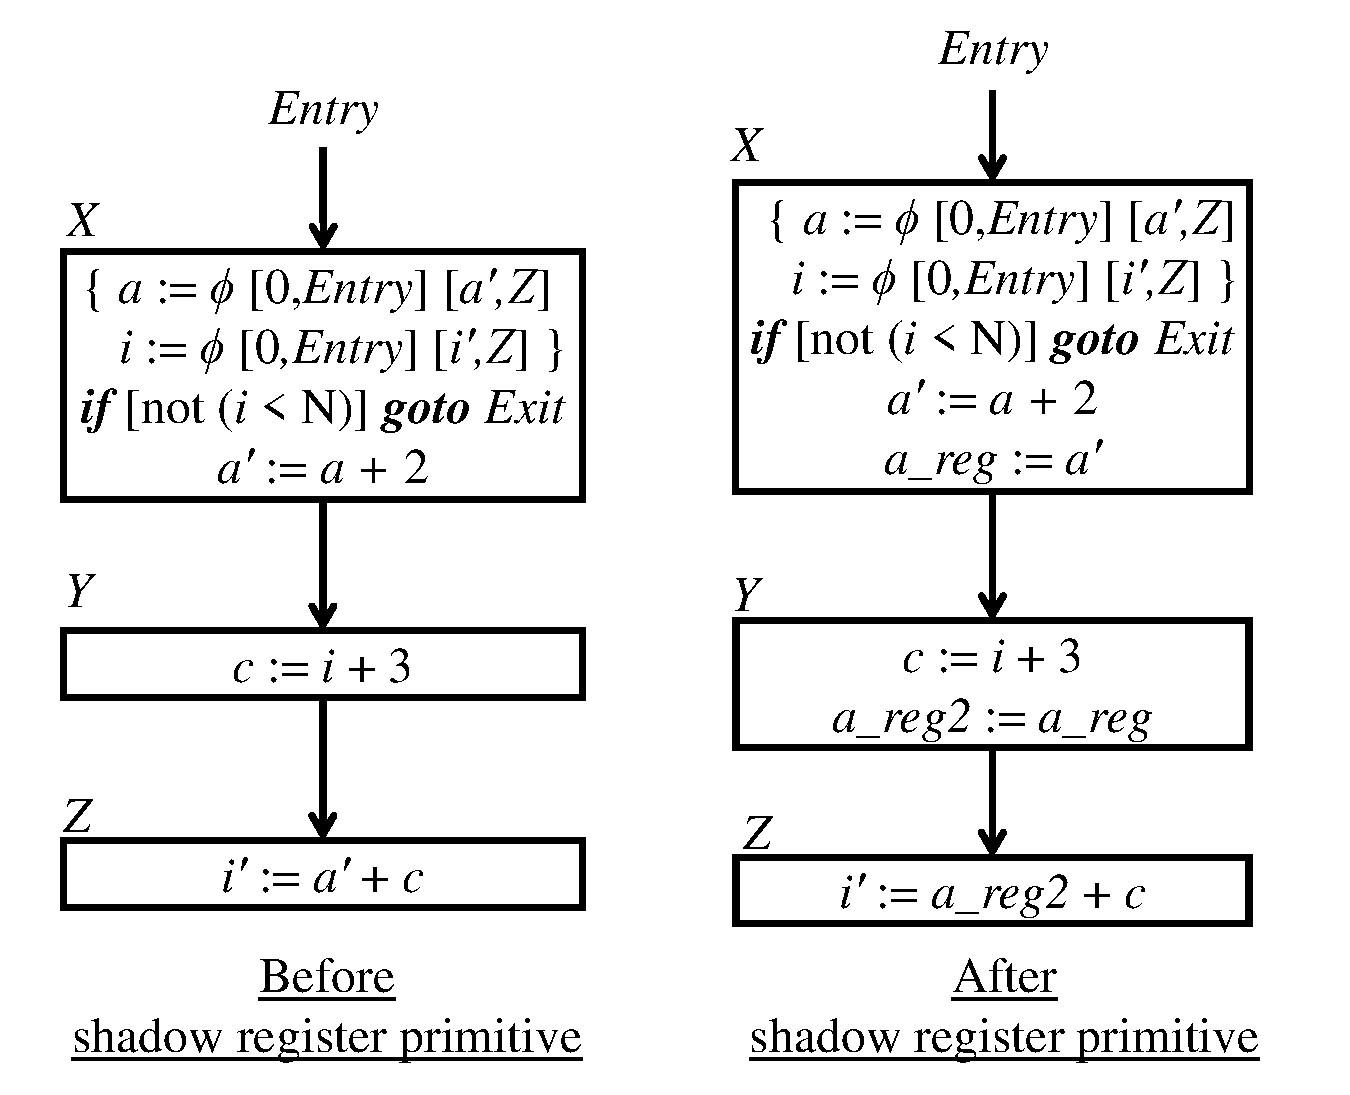
\includegraphics[height=2.2in]{fig-proposal/shadow-reg-primitive}
\end{center}
\caption{Shadow Register Primitive}
\label{fig:primitives1}
\end{figure}

{\textbf {Shadow register primitive}} -- We define a shadow register microstep as simply an assignment
statement with symbol expression ($x$) assigned to a new value ($x\_reg$). We call all the new introduced variables as shadow registers. Intuitively, it is correct that in a
sequence of steps, if we assign a variable to a shadow register and replace all occurences of $x$ with $x\_reg$
till the next write of $x$, we should
not have made any difference in the execution. Also, since we are not changing the value of $x$ itself,
 the state after end of execution for both CCDFGs as far as real variables are concerned (all variables
 excluding all shadow registers) is same. In Figure~\ref{fig:primitives1}, if we assign a shadow register
 $a\_reg$ value of $a'$ at the end of $X$ block, shadow register $a\_reg2$ value of $a\_reg$ in $Y$ and replace the read occurence of $a'$ in $Z$ with $a\_reg2$, the sequential execution remains same.
But, because of the addition of these shadow registers, the value of $a'$ is stored in a new temporary variable in every new scheduling step which prevents data hazards.

{\textbf {Interchange primitive}} -- Let $m$ and $n$ be two adjacent scheduling steps (or in general, any collection of microsteps) in a CCDFG where both $m$ and $n$ do not have any microsteps containing branch statements. Also, there are no read write hazards between $m$ and $n$. By read write hazards, we mean that $m$ does not read or write any variable which is written in $n$ and vice versa. Then, the interchange primitive allows us to interchange the order of $m$ and $n$ in the given CCDFG. Note that under the given assumptions, if initial state is the same, then the state reached after executing $m$ followed by $n$ is same as the state reached after executing $n$ followed by $m$.

\begin{figure}[t!]
\begin{center}
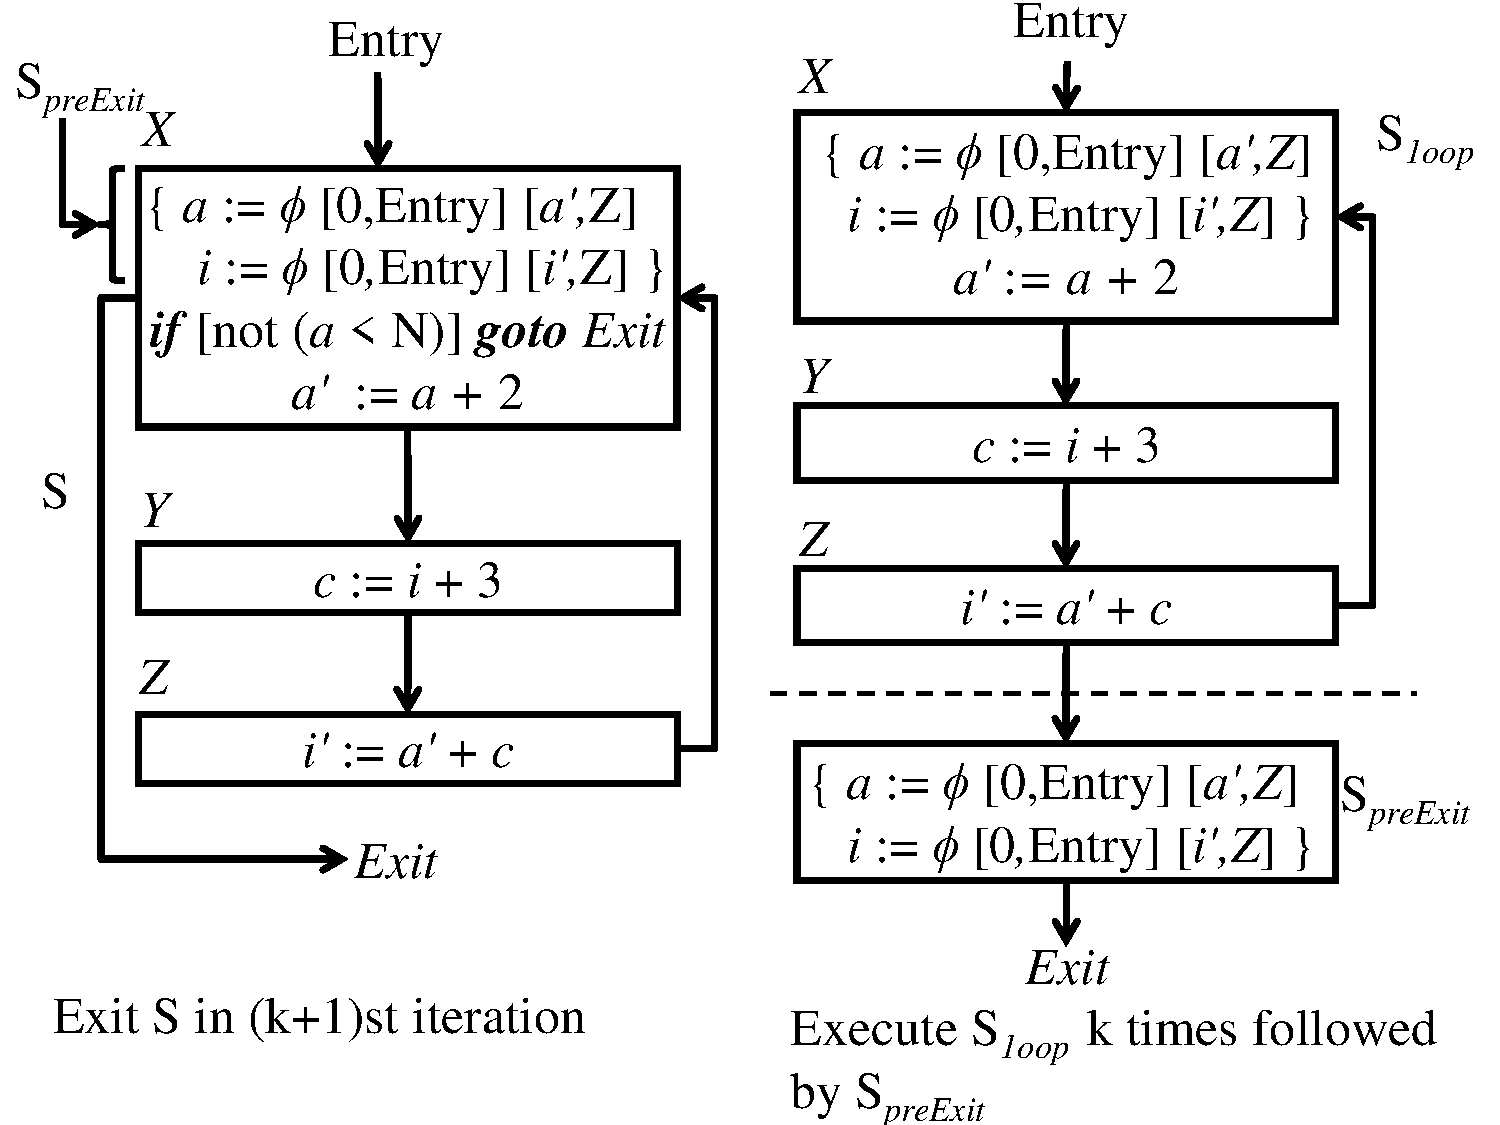
\includegraphics[height=2.2in]{fig-proposal/conditional-branch-primitive}
\end{center}
\caption{Conditional Branch Primitive}
\label{fig:primitives2}
\end{figure}

{\textbf {Conditional branch primitive}} -- Branch instructions are required to determine the control flow. However,
reasoning semantically about conditional branch instructions in a loop everytime we apply a primitive can make proof very complex. We have to always keep track of condition variable to make sure that loop exits if the condition is true.
We note that if we specifically assume that the exit condition becomes true after completing $k$ iterations, then we can remove the conditional branch.
To understand the conditional branch primitive (c.f. Figure~\ref{fig:primitives2}), 
let's assume there is a conditional branch in the sequential loop structure $S$, which points to either
the next microstep in sequence or exits the loop by branching to the scheduling step
$Exit$. Let $S_{preExit}$ be the collection of microsteps before this branch in $S$ and
let $S_{loop}$ be the corresponding CCDFG loop without the conditional branch.
The conditional branch primitive allows us to replace $S$ with $S_{loop}$ followed by
$S_{preExit}$. Similarly,
the primitive also allows us to introduce an exit conditional branch by replacing
$S_{loop}$ followed by $S_{preExit}$ with $S$.
Note that since $k$ can take any value $k \ge 0$, we are not compromising on the correctness statement.  
It can be proved that executing $S$ $k$ times such that it exits in the $(k+1)$ st
iteration is same as executing $S_{loop}$ $k$ times followed by $S_{preExit}$.

{\textbf {Superstep construction primitive}} -- This operation entails combining the scheduling steps of the successive
iterations, forming scheduling ``supersteps'' that act as scheduling steps for the pipelined implementation. Supersteps must
account for read-after-write hazards, i.e, if a variable is written in a scheduling step $X$ and read subsequently in
$Z$ then $Z$ cannot be in a superstep that precedes $X$ in the control/data flow.  Note that we implement data
forwarding (forward value of data within a single clock cycle); thus $X$ and $Z$ can be in a single superstep.

\section{Our Loop Pipelining Algorithm}
Given a sequential loop $S$ in CCDFG $C$ and pipeline interval $I$, we can create a pipelined loop $P$ using Algorithm~\ref{algo:disha}. Note that every step of the algorithm is build from ground up using our framework of provable primitives such that the algorithm can be certified by theorem proving.

{\bf Note to Disha: Showing errors in printing algorithms. Trying to debug}
%\begin{algorithm}[H]
	%\caption{Pipelining Algorithm}
	%\label{algo:loop}
	%\begin{algorithmic}[1]
		%\Procedure{PipelineLoop}{S, I}
		%\State $S_1 \leftarrow RemoveBranches(S)$
		%\State $S_2 \leftarrow UnrollLoopOnce(S_1)$
		%\State $S_3 \leftarrow \phi-Elimination (S_2) $.
		%\State $S_4 \leftarrow DataPropagation (S_3, I) $.
		%\State $S_5 \leftarrow GenerateShadowRegisters (S_4, I) $.
		%\State $ S_6 \leftarrow SuperstepConstruction (S_5, I) $.
		%\State $P \leftarrow AddBranches (S_6) $
		%\State \textbf{return} $(P)$.
		%\EndProcedure
	%\end{algorithmic}
%\end{algorithm}

%
%x

Below we describe the steps to convert a sequential loop CCDFG to a pipelined loop CCDFG in detail:
 
{\bf Remove Branches}: We apply the branch primitive on $S$ (c.f. Figure~\ref{fig:algo1}(a)) to remove the conditional and unconditional branch by explicitly defining the control flow in $S$. The output is a sequence of two CCDFG's $S_{loop}$ and $S_{Exit}$ connected through an edge as shown in Figure~\ref{fig:algo1}(b).
Note, that $S_{loop}$ does not contain the conditional branch originally present in $S$.
Executing $S$ such that $S$ exits in the $(k+1)$st iteration is semantically same as executing $S_{loop}$ $k$ times
followed by $S_{preExit}$. This is possible because the input CCDFG has only one conditional and one unconditional branch as per our definition of well-formed-ccdfg 

{\bf Unroll Loop Once}: We have already established that the first iteration behaves differently than the rest of the
iterations due to $\phi$-construct. So, here we simply unroll the loop $S_{loop}$ once. We call the first iteration
$S_{pre}$ as shown in Figure~\ref{fig:algo1}(c).

\begin{figure}[t!]
\begin{center}
\begin{tabular}{ccc}
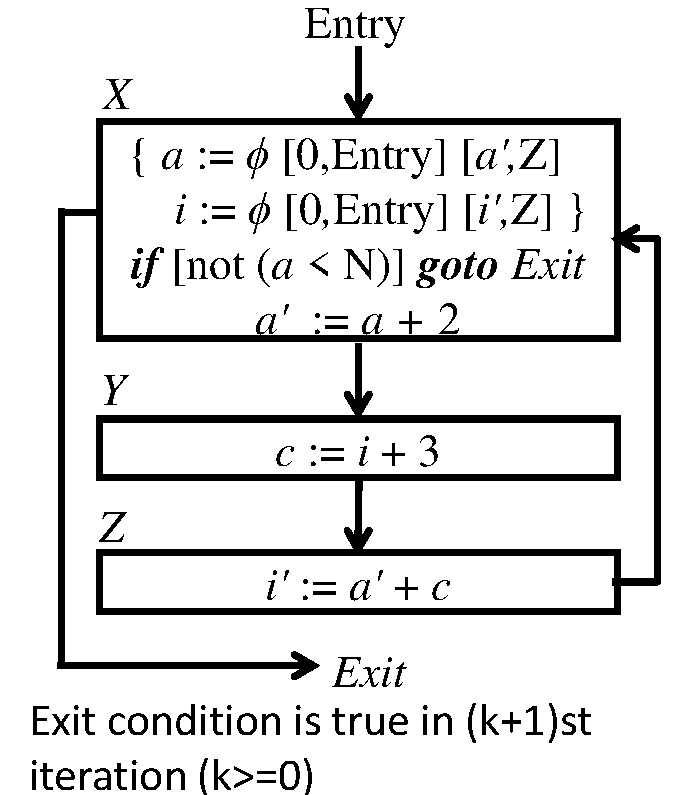
\includegraphics[height=1.6in]{fig-proposal/seq-ccdfg}
&
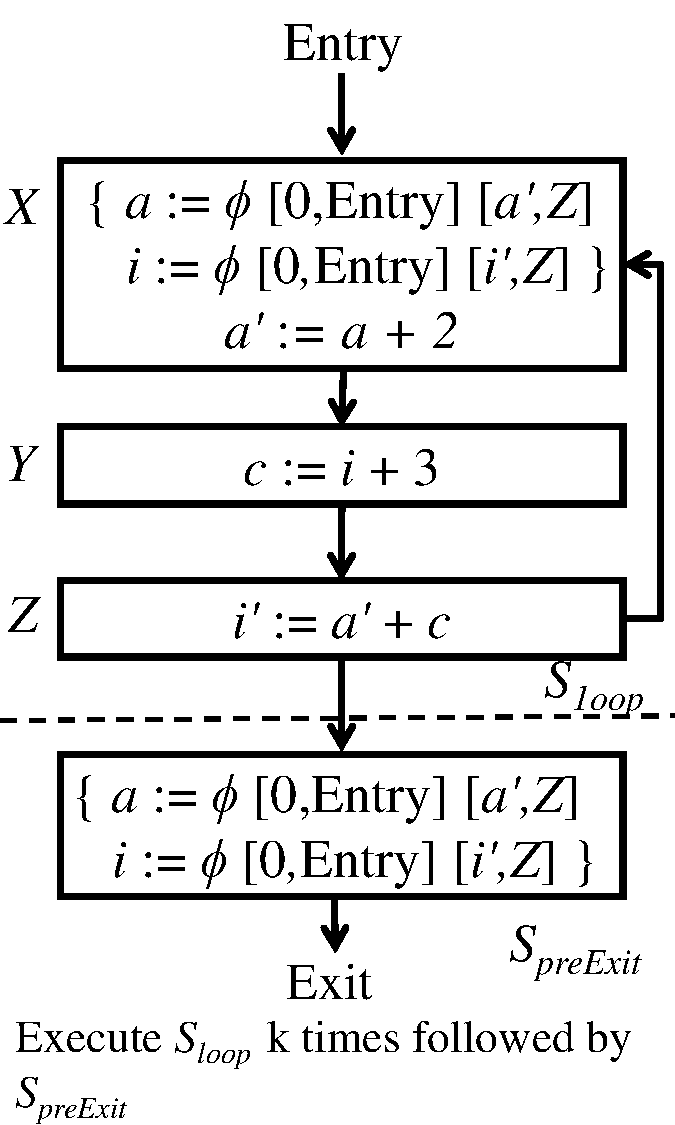
\includegraphics[height=2.5in]{fig-proposal/algorithm-after-removing-branches}
&
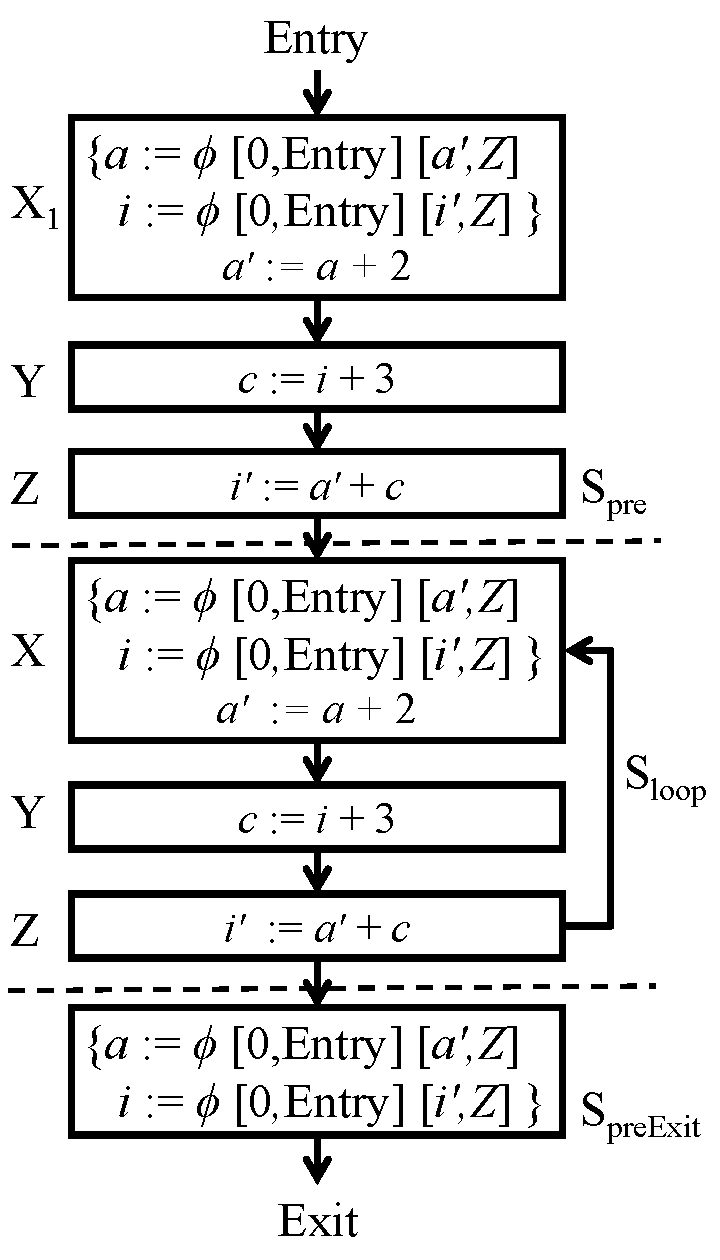
\includegraphics[height=2.5in]{fig-proposal/algorithm-two-iterations}
\\
(a) & (b) & (c)
\end{tabular}
\end{center}
\caption{(a) Sequential CCDFG with conditional branch (b) Sequential CCDFG without conditional branch. Note the addition of $S_{Exit}$ to explicitely define the control flow (c) Unrolling the loop once to separate the first iteration}
\label{fig:algo1}
\end{figure}

{\bf $\phi$-elimination}: We apply the $\phi$-elimination primitive on $S_{pre}$, $S_{loop}$ and $S_{Exit}$ to return a CCDFG in which all the $\phi$-statements have been replaced with their corresponding assignment statements. Figure~\ref{fig:algo2}(a) shows the CCDFG after applying the $\phi$-elimination primitive. Note that $\phi$-construct is only in the first scheduling step of any iteration, so the remaining scheduling steps are the same in all the iterations.

{\bf Data propagation:} Algorithm~\ref{algo:data-propagation} describes how to compute candidates for data
propagation across pipeline iterations. It is a critical step in removing data hazards. We want to make sure that when we pipeline a loop, we do not read a variable which has not
yet been written. A critical observation is that data propagation is required only for loop carried dependencies.
$GetLoopCarriedDependencies$ identifies the microsteps where loop carried dependencies are being read. Then,
$CheckConflict$ checks whether there would be a conflict when we pipeline the loop.
Conflict occurs when the value being read in a microstep is not yet written in the pipelined loop execution. If so, $RelocateMSteps$ works in two steps. It first relocates the microstep which reads the variable in an iteration to the starting of $S_{loop}$. This step can be proved by the interchange primitive since we have already established that the value has not been written yet so there are no read write hazards in between. In the next step, we relocate the microstep to the end of $S_{loop}$. Note, to maintain the invariant that executing CCDFG semantically before and after this relocation is the same, we need to add the microstep at the end of $S_{pre}$ as well and remove it from $S_{Exit}$. This step ensures that any variable which is being read has already been written. Note that in order to maintain the invariant, only those microsteps can be propagated which exist in $S_{Exit}$, which means only those steps which occur before the conditional branch in original CCDFG can be relocated. This ensures that our algorithm does not have the bug which the previously proposed algorithm had.
In Figure~\ref{fig:algo1}(c) we found that the loop carried dependency $i'$ in $X$ would create a conflict when we would move $X$ before $Z$ while pipelining. So, first we relocate the microstep $i := i'$ to the beginning of $S_{loop}$ using interchange primitive in Figure~\ref{fig:algo2}(b). Then, we move the microstep to end of $S_{pre}$ and $S_{loop}$ and remove the microstep from $S_{Exit}$ in  Figure~\ref{fig:algo2}(c). Note that this preserves semantic equivalence.
This step needs to be repeated for every variable found using $GetLoopCarriedDependencies$.


%\begin{algorithm}[H]
%\caption{Data propagation} \label{algo:data-propagation}
%\begin{algorithmic}[1]
%\Procedure{DataPropogration}{$L$}
%\State $msteps \leftarrow GetLoopCarriedDependencies(L)$.
%\For {\textbf{each} mstep \textbf{in} msteps}
 %\If {$CheckConflict (L, mstep, N, I) \neq 0$}
%\State $L \leftarrow RelocateMStep (L, mstep)$.
%\EndIf
%\EndFor
%\State \textbf{return} $(L)$.
%\EndProcedure
%\end{algorithmic}
%\end{algorithm}

\begin{figure}[t!]
\begin{center}
\begin{tabular}{ccc}
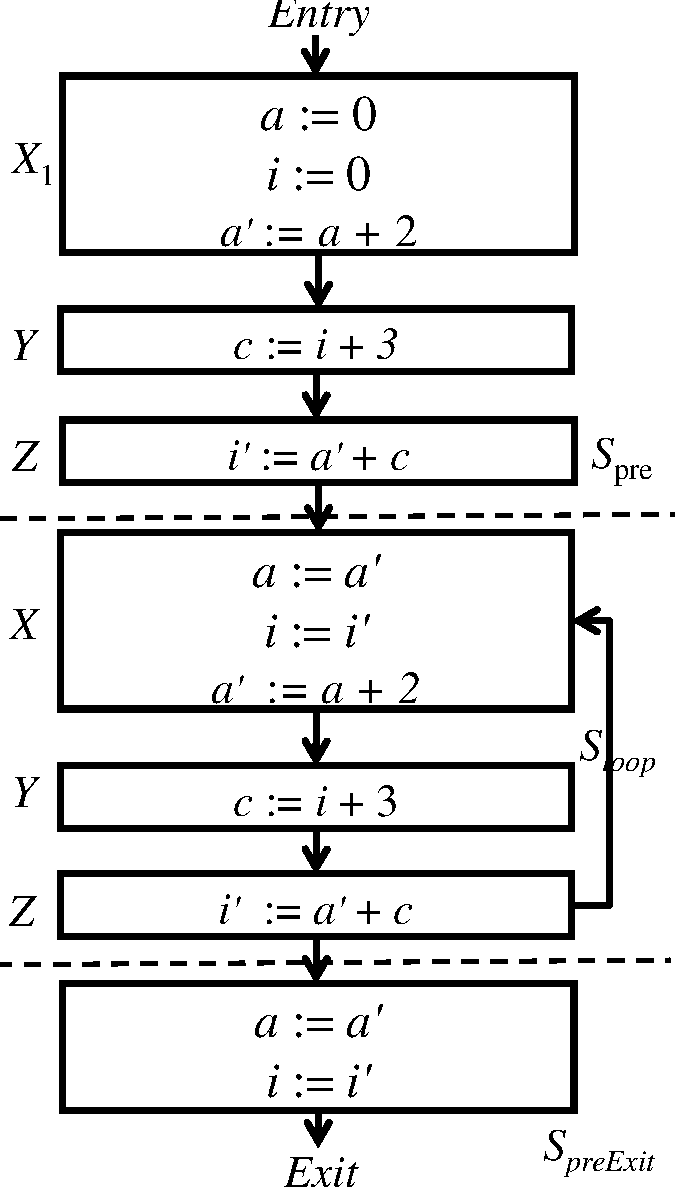
\includegraphics[height=2.5in]{fig-proposal/algorithm-after-phi-removal}
&
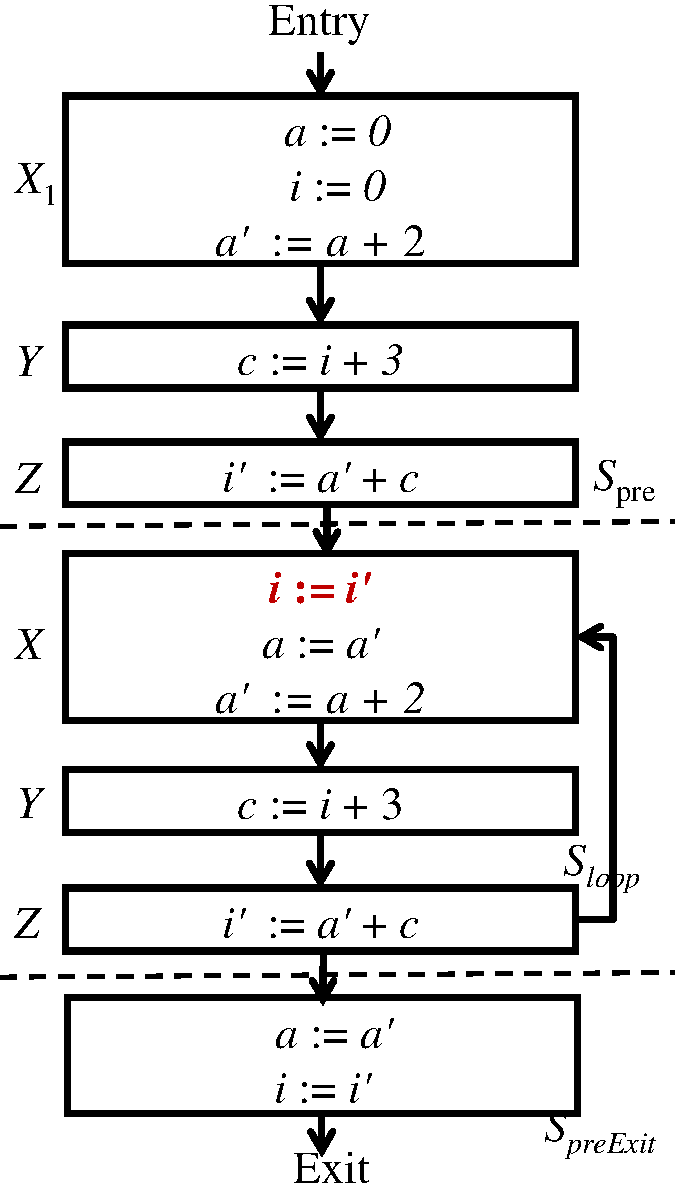
\includegraphics[height=2.5in]{fig-proposal/algorithm-after-data-propagation-1}
&
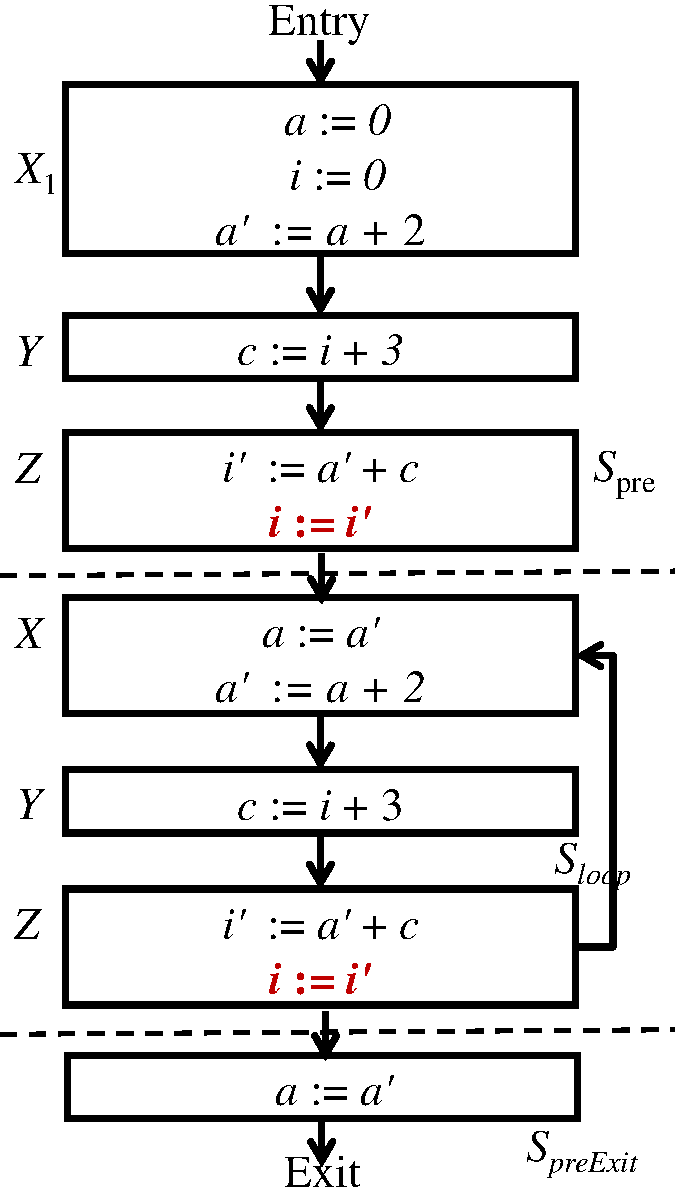
\includegraphics[height=2.5in]{fig-proposal/algorithm-after-data-propagation-2}
\\
(a) & (b) & (c)
\end{tabular}
\end{center}
\caption{(a) After $\phi$-removal transformation (b) Data propagation - first step (c) Data Propagation - second step}
\label{fig:algo2}
\end{figure}

{\bf Generate shadow registers:} Algorithm~\ref{algo:generate-pipeline-registers} inserts shadow registers
to prevent variables from being overwritten before being read. We first compute all program variables that may be
overwritten before being read, which means these are the variables that require shadow registers. To find such variables,
 $GetAllVariables$ first gets a set of all variables. Then, for each variable, we compare the distance between the write of
  the variable $w_v$ $(WriteVariable)$ and the last read of the variable $r_v$ $(LastReadVariable)$ in an iteration; if the
   distance is greater than $I$, the variable is assigned the new data value of the next iteration before the current iteration's value
    has been fully consumed; this warrants insertion of shadow registers in every scheduling step between the $r_v$ and $w_v$. The value is propagated every clock cycle following the CCDFG data flow.
We apply the shadow register primitive on the microstep which writes the variable $(AddShadowRegister)$. We assign that
 variable to a new temporary variable called shadow register in every new scheduling step and replace all subsequent reads of that variable with the shadow register till its next write. In Figure~\ref{fig:algo3} (a), we introduce a shadow register $a\_reg$ in $X$ and $a\_reg2$ in $Y$. This step is also repeated for all the variables found using $GetAllVeriables$.

%\begin{algorithm}
%\caption{Generate shadow registers} \label{algo:generate-pipeline-registers}
%\begin{algorithmic}[1]
%\Procedure{GenerateShadowRegisters}{$L$}
%\State $V \leftarrow GetAllVariables(L)$.
%\For {\textbf{each} v \textbf{in} V}
%\State $w_v \leftarrow WriteVariable (v, L)$.
%\State $r_v \leftarrow LastReadVariable (v, L)$.
%  \If {$RequireShadowRegister (r_v, w_v, I) \neq 0$}
%\State $L \leftarrow AddShadowRegister (w_v, L)$.
%\EndIf
%\EndFor
%\State \textbf{return} $(L)$.
%\EndProcedure
%\end{algorithmic}
%\end{algorithm}

\begin{figure}[t!]
\begin{center}
\begin{tabular}{cc}
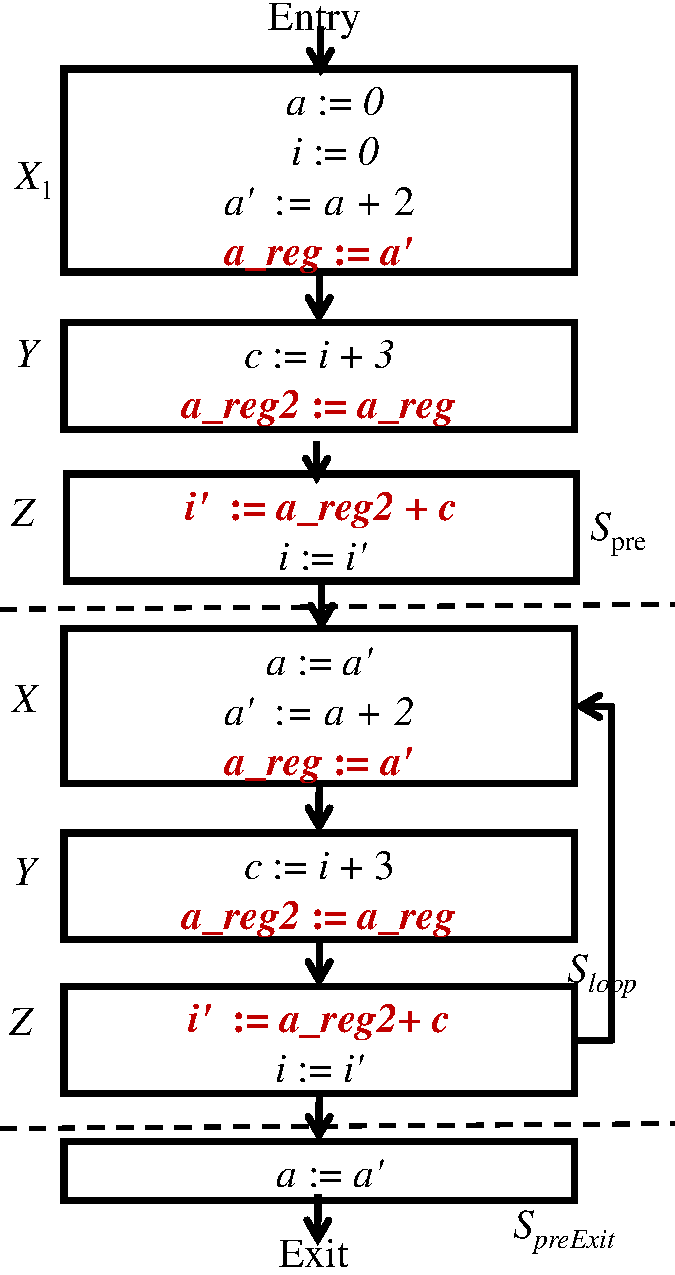
\includegraphics[height=2.5in]{fig-proposal/algorithm-after-shadow-register}
&
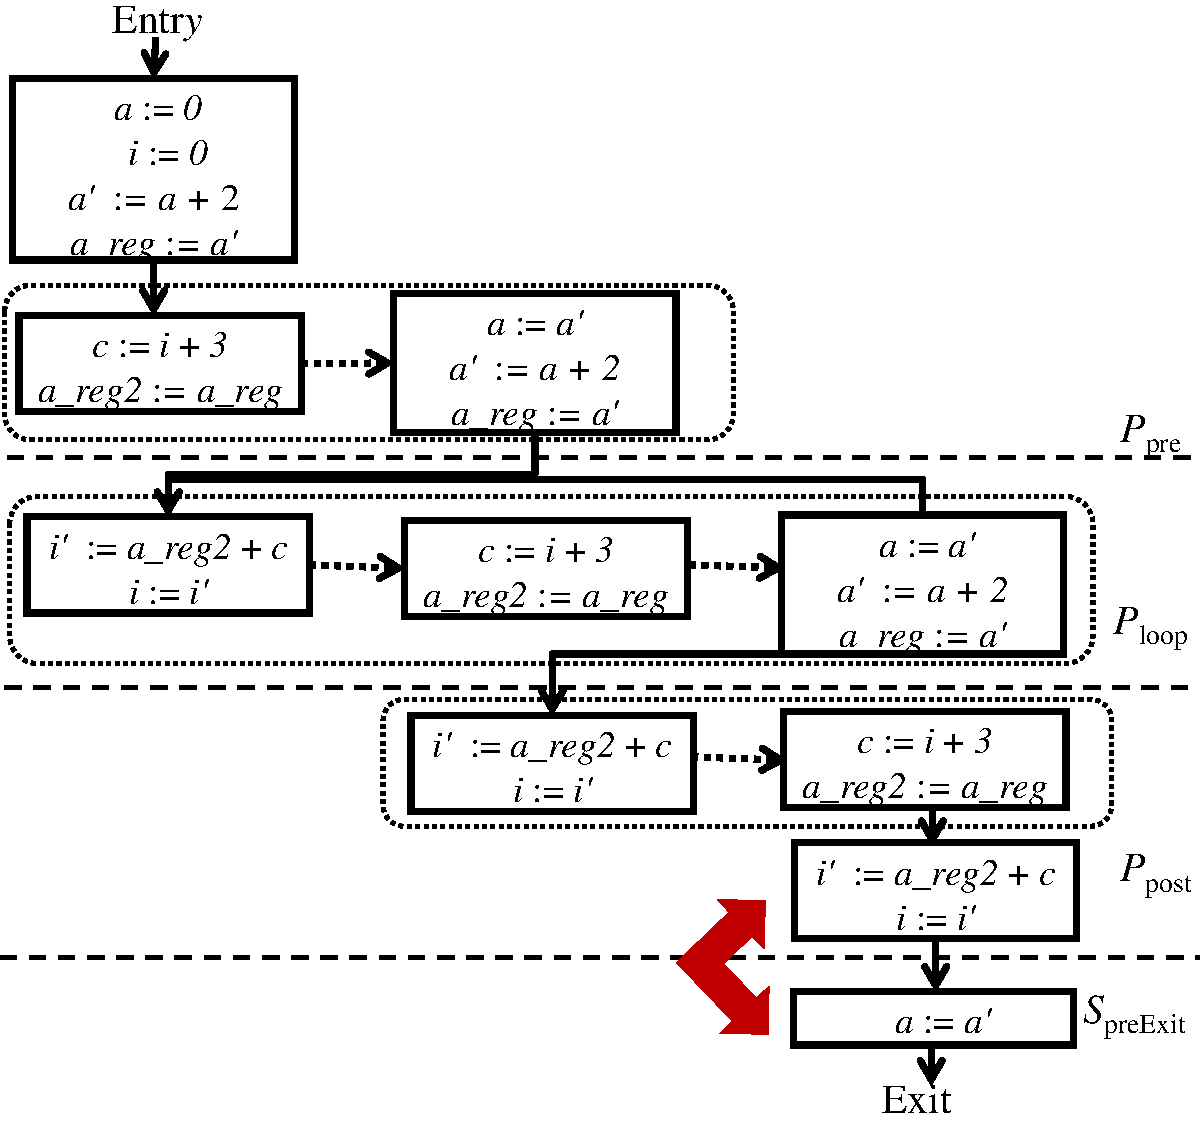
\includegraphics[height=2.5in]{fig-proposal/algorithm-after-superstep-construction}
\\
(a) & (b)
\end{tabular}
\end{center}
\caption{(a) After shadow register transformation (b) After superstep construction}
\label{fig:algo3}
\end{figure}

{\bf Superstep construction:} Now that we have removed the data hazards, we can successfully pipeline the loop using  the pipeline interval $I$. We combine the scheduling steps of the successive iterations, forming scheduling ``supersteps'' that act as scheduling steps for the pipelined
implementation. Supersteps must account for read-after-write hazards, i.e., if a variable is written in a scheduling step $s$ and read subsequently in $s'$ then $s'$ cannot be in a superstep that precedes $s$ in the control/data flow. A scheduling step is allowed to move up another scheduling step only if there are no intermediate read and write conflicts. Note that we implement data forwarding; thus $s$ and $s'$ can be in a single scheduling superstep.
Superstep construction on $S_{pre}$ and $S_{loop}$ creates a CCDFG with three parts: prologue $P_{pre}$, $P_{loop}$ which is the full pipeline stage and epilogue $P_{post}$ as shown in Figure~\ref{fig:algo3} (b). We will later prove using our invariant that executing $P_{pre}$ followed by $k$ iterations of $P_{loop}$ followed by $P_{post}$ is equivalent to executing $S_{pre}$ followed by $x$ iterations of $S_{loop}$, where value of $x$ is determined based on value of $k$, pipeline interval $I$ and number of scheduling steps in $S$.

\begin{figure}[t!]
\begin{center}
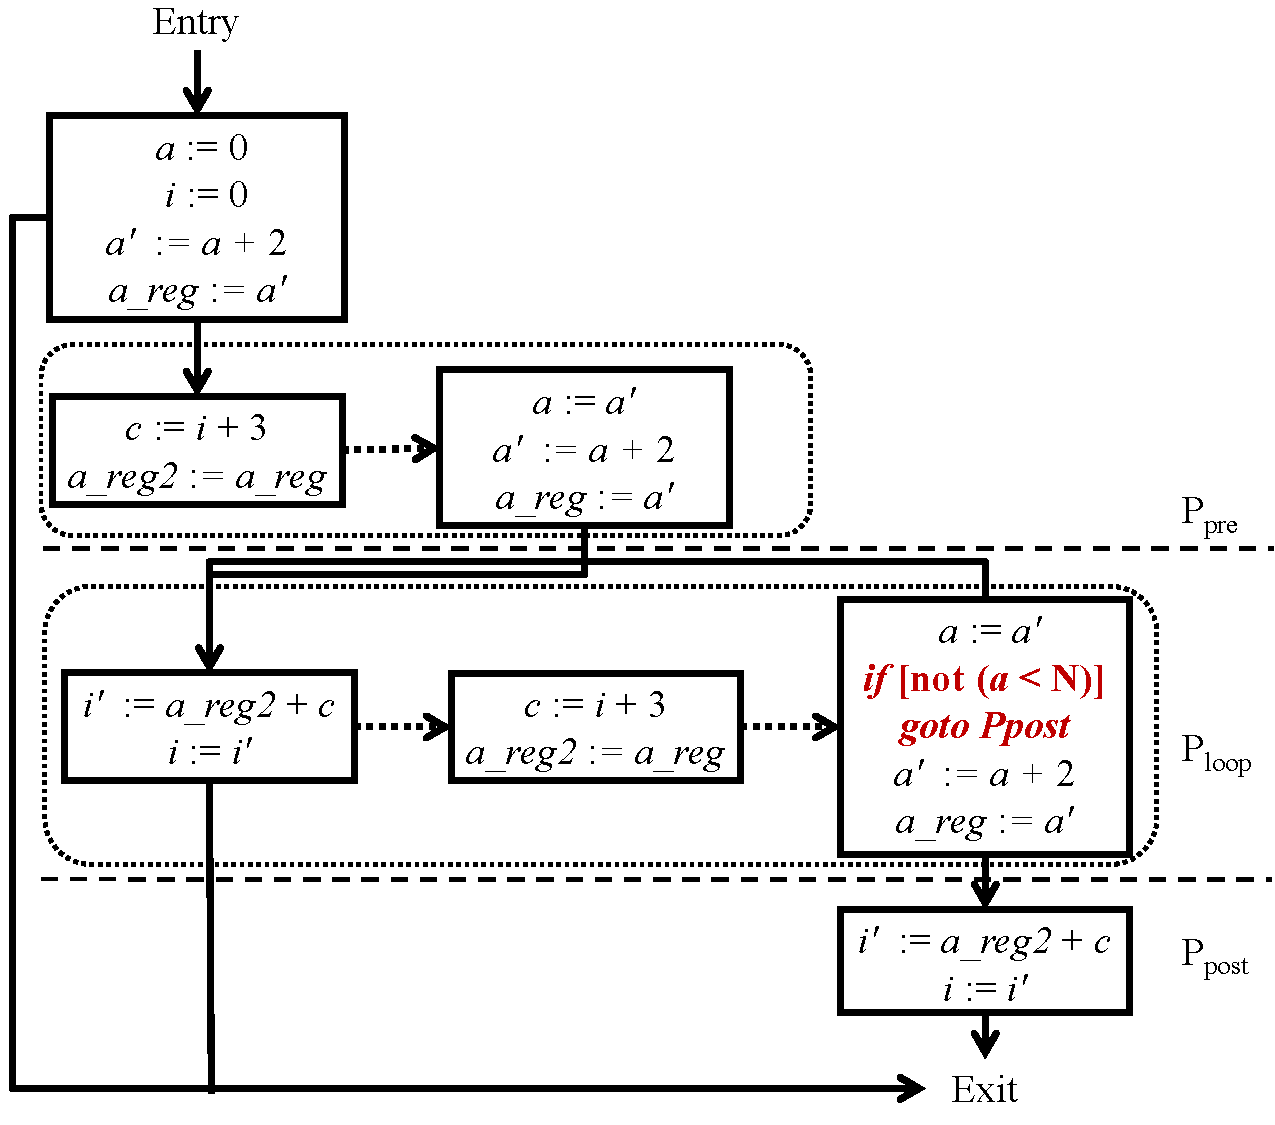
\includegraphics[height=2.5in]{fig-proposal/algorithm-after-adding-branches}
\end{center}
\caption{Final Pipelined CCDFG}
\label{fig:algo4}
\end{figure}

{\bf Add Branches:}  To add the branches back, we use the a combination of interchange primitive and reverse of Branch primitive. Note in Figure~\ref{fig:algo3}(b), if there are no read write hazards in between the last scheduling step $Z$ of $P_{post}$ and $S_{Exit}$, we can interchange them using interchange primtive. Now recall from the branch primitive that if there is a loop structure, here $P_{loop}$ followed by a collection of microsteps from the beginning of $P_{loop}$ in sequence, say $P_{Exit}$ (here, a collection of $Z$, $Y$ and $S_{Exit}$), then we can add an exit conditional branch in $P_{loop}$ after the microsteps $P_{Exit}$ which exits the loop and points to the next scheduling step after the loop if the exit condition is true. We can add the conditional and the unconditional branch as shown in  Figure~\ref{fig:algo4}.  

%Next we discuss an outline of the proof of our algorithm using theorem proving. 